\section{TensorBoard}
\begin{python}
import tensorflow as tf
import numpy as np

tf.set_random_seed(1)
np.random.seed(1)

# fake data
x = np.linspace(-1, 1, 100)[:, np.newaxis]          # shape (100, 1)
noise = np.random.normal(0, 0.1, size=x.shape)
y = np.power(x, 2) + noise                          # shape (100, 1) + some noise

with tf.variable_scope('Inputs'):
        tf_x = tf.placeholder(tf.float32, x.shape, name='x')
        tf_y = tf.placeholder(tf.float32, y.shape, name='y')
with tf.variable_scope('Net'):
    l1 = tf.layers.dense(tf_x, 10, tf.nn.relu, name='hidden_layer')
    output = tf.layers.dense(l1, 1, name='output_layer')
    tf.summary.histogram('h_out', l1)
    tf.summary.histogram('pred', output)
    loss = tf.losses.mean_squared_error(tf_y, output, scope='loss')
    train_op = tf.train.GradientDescentOptimizer(learning_rate=0.5).minimize(loss)
    tf.summary.scalar('loss', loss)     # add loss to scalar summary

    sess = tf.Session()
    sess.run(tf.global_variables_initializer())

    writer = tf.summary.FileWriter('./log', sess.graph)     # write to file
    merge_op = tf.summary.merge_all()                       # operation to merge all summary

    for step in range(100):
        _, result = sess.run([train_op, merge_op], {tf_x: x, tf_y: y})
        writer.add_summary(result, step)
\end{python}
\begin{figure}[H]
	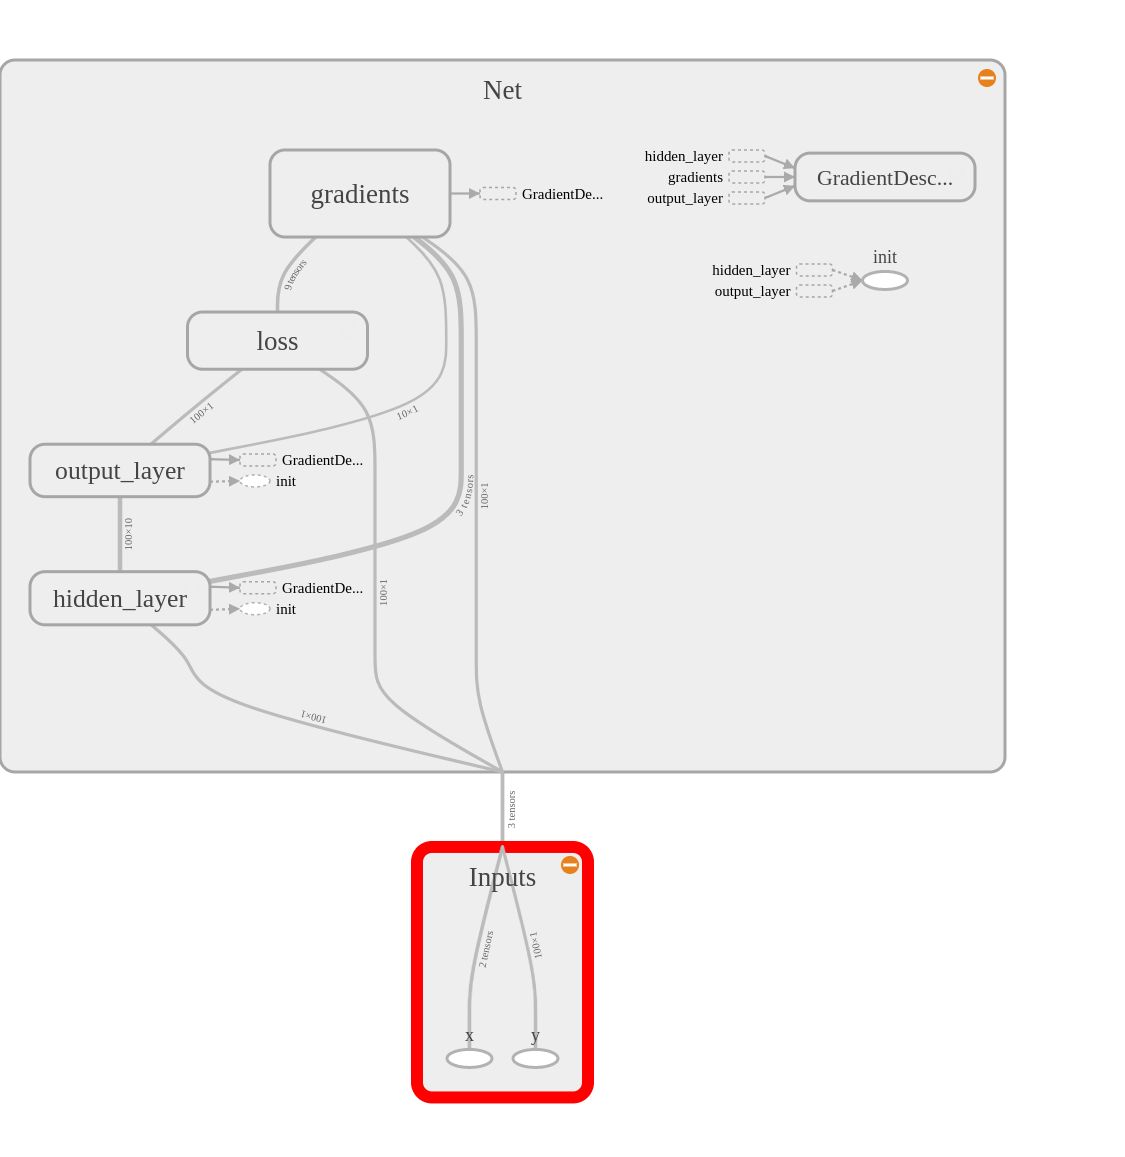
\includegraphics[scale=0.4]{./pic/chapter1/tenbor1.png}
\end{figure}

